\documentclass[../main.tex]{subfiles}

\begin{document}
\begin{problema}
	Considere una cadena de longitud \(L\) y densidad de masa \(\rho\) por
	unidad de longitud. La cadena está apila sobre una mesa fija como
	se muestra en la figura. Determinar la fuerza \(\boldvect\vect{F}\)
	necesaria para levantar la cadena a una velocidad \(\boldvect\vect{\nu}\). Considere
	que hay gravedad.

	\begin{figure}[htb]
		\centering
		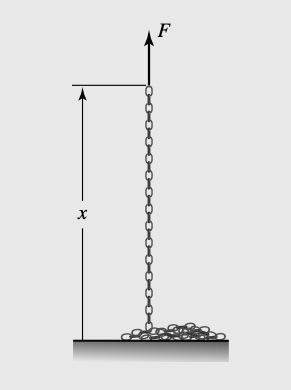
\includegraphics[width=.3\textwidth]{figs/problema01-000.jpg}
	\end{figure}
\end{problema}

\startsolution

De la segunda ley de Newton tenemos que

\begin{equation}
	F + F_{g} = \int_{\Omega} \pdv{\rho \vect{v}}{t} \odif{v} + \int_{\pdif{V}} (\rho \vect{v})\cdot \vect{v} \cdot \odif{\vect{S}}.
	\label{eq:NewtonSecondLaw}
\end{equation}

La fuerza debida a la aceleración de la gravedad es

\begin{equation*}
	F_{g} = -\rho gx.
\end{equation*}

Entonces, la \zcref{eq:NewtonSecondLaw} queda de la siguiente manera por
ser un problema unidimensional,

\begin{equation*}
	F - \rho gx = \pdv{(\rho v)}{t} + \rho v^{2}.
\end{equation*}

Y como \(v\) es constante,

\begin{align*}
	F             & = \rho gx + \rho v^{2}, \\
	\Aboxedmain{F & = \rho(gx + v^{2}).}
\end{align*}
\end{document}
